\documentclass{article}

% Language setting
% Replace `english' with e.g. `spanish' to change the document language
\usepackage[english]{babel}

% Set page size and margins
% Replace `letterpaper' with `a4paper' for UK/EU standard size
\usepackage[a4paper,top=2cm,bottom=2cm,left=3cm,right=3cm,marginparwidth=1.75cm]{geometry}

% Useful packages
\usepackage{amsmath}
\DeclareMathOperator{\sinc}{sinc}

\usepackage{amssymb}

\usepackage{graphicx}
\usepackage[colorlinks=true, allcolors=blue]{hyperref}


\usepackage{tikz}
\usetikzlibrary{arrows,decorations.pathmorphing,backgrounds,fit,positioning,shapes.symbols,chains,shapes.geometric,shapes.arrows,calc}


\usepackage{listings}
\usepackage{xcolor}
\usepackage{enumitem}
\usepackage{physics}
\setlist[itemize]{nosep} 

\definecolor{codegreen}{rgb}{0,0.6,0}
\definecolor{codegray}{rgb}{0.5,0.5,0.5}
\definecolor{codepurple}{rgb}{0.58,0,0.82}
\definecolor{backcolour}{rgb}{0.95,0.95,0.92}

\lstdefinestyle{mystyle}{
    backgroundcolor=\color{backcolour},   
    commentstyle=\color{codegreen},
    keywordstyle=\color{magenta},
    numberstyle=\tiny\color{codegray},
    stringstyle=\color{codepurple},
    basicstyle=\ttfamily\footnotesize,
    breakatwhitespace=false,         
    breaklines=true,                 
    captionpos=b,                    
    keepspaces=true,                 
    numbers=left,                    
    numbersep=5pt,                  
    showspaces=false,                
    showstringspaces=false,
    showtabs=false,                  
    tabsize=2
}

\lstset{style=mystyle}


\title{Homework 1, Reti Di Calcolatori}
\author{Matteo Galiazzo}

\begin{document}
\maketitle

\tableofcontents

\section{Scelta dell'immagine}

Per questo homework è stata scelta l'immagine \verb|einst.pgm|, ma sono state usate anche altre immagini per verificare la correttezza delle ipotesi.
L'immagine è:
\begin{figure}[h]
    \centering
    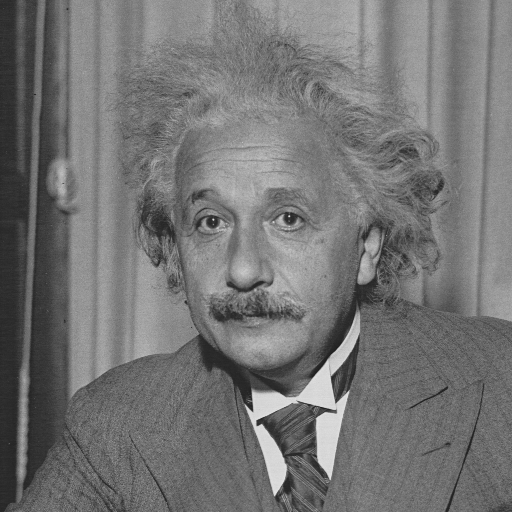
\includegraphics[width=0.4\linewidth]{einst.png}
    \caption{einst.pgm}
    \label{fig:einst_pgm}
\end{figure}

\section{Confronto tra entropia e tasso di codifica}

Non possiamo fare una comparazione quantitativa ma possiamo dire che:
\begin{itemize}
    \item \textbf{Immagini con entropia alta}: hanno una distribuzione dei valori dei pixel più uniforme, che rende più difficile la compressione.
    Questo perchè il compressore ha bisogno di salvare più informazione per rappresentare la casualità dei pixel nell'immagine.
    Come risultato il tasso di compressione è più basso, e la dimensione dell'immagine compressa è più alta.
    
    \item \textbf{Immagini con entropia bassa}: hanno uan distribuzione dei valori dei pixel più strutturata, che rende più facile la compressione.
    Il compressore sfrutta la predicibilità dei pixel nell'immagine per rappresentarla in modo più efficiente, risultando in un tasso di compressione più alto, e la dimensione dell'immagine compressa è più bassa.
\end{itemize}

Nella nostra immagine il rapporto di compressione ottenibile di $1.179 \, bpp$ ci indica che abbiamo un'entropia alta.

\section{Confronto tra codifica Exp Golomb con segno e codifica predittiva semplice}

La codifica di Exp Golomb funziona bene quando i dati sono sparsi, nel punto precedente abbiamo visto che abbiamo un'alta entropia nell'immagine e quindi Exp-Golomb funziona bene, infatti l'entropia dell'errore di predizione per l'immagine scelta con la codifica semplice è $5.399 \, bpp$ (bits per pixel) e il rapporto di compressione ottenibile è $1.48$.
Una volta che abbiamo effettuato la compressione semplice possiamo calcolare il tasso di codifica sull'errore di predizione usando exp-golomb con segno, e otteniamo $6.946 \, bpp$.

\section{Confronto tra codifica Exp Golomb con segno e codifica predittiva avanzata}

% Valutare il numero di bit necessari per codificare l’errore di predizione con la codifica Exp Golomb con segno, dedurne il tasso di codifica e confrontare tale valore con quello ottenuto ai punti 1,3 e 5

Per codificare l'errore di predizione della foto scelta con la codifica di Exp Golomb con segno servono $1709902 \, bit$.

Possiamo dedurre da questo il tasso di codifica con un semplice conto:
$ \text{tasso codifica} = \frac{\text{bit codifica}}{\text{numero pixel}} = 6.523 \, bpp$

Usando la codifica avanzata otteniamo un numero di bit per pixel più basso della codifica semplice, ma non di molto.
Questo è sensato perchè inizialmente abbiamo trovato un'entropia alta sull'immagine, quindi ci aspettiamo di non riuscire a comprimere molto bene (usando pochi bit per pixel) neanche con un metodo di codifica avanzato

\section{Valori di output del programma}

\begin{lstlisting}
===== einst.pgm =====
Entropy of the image: 6.785001977240487
The theoretical compression rate is: 1.1790711376113205
The image has 262144 pixels
--- simple predictive encoding ---
The entropy of the encoded image is: 5.180007934203807
The obtainable compression rate is: 1.544399178845976
bit per pixel con codifica exp_golomb: 6.946563720703125
--- advanced predictive encoding ---
image shape: (512, 512)
pixel count: 262144
The entropy of the encoded image is: 4.785572850353761
The obtainable compression rate is: 1.671691195633689
bit count: 1709902
bit per pixel con codifica exp_golomb: 6.522758483886719
\end{lstlisting}

\newpage 
\section{Codice python della codifica predittiva avanzata}

\begin{lstlisting}[language=python]
def advanced_predictive_encoding(img):
    rows, cols = img.shape
    print(f"image shape: {img.shape}")
    print(f"pixel count: {rows * cols}")

    prediction = np.zeros((rows, cols))
    prediction[0, 0] = img[0, 0] - 128

    # for each pixel in position n, m
    # first row -> predictor left from current pixel
    # first column -> predictor on top of current pixel
    # last column -> predictor is the median value between x(n-1, m), x(n,m-1) and x(n-1, m-1)
    # else -> predictor is the median value between x(n-1, m) x(n, m-1), x(n-1, m+1)
    # once the predictor is built you can calculate the prediction error y = x-p (it's an image)

    n = 0
    while n < rows:
        m = 0
        while m < cols:
            # first row
            if n == 0:
                prediction[n, m] = img[n, m - 1]
            # first column
            elif m == 0:
                prediction[n, m] = img[n - 1, m]
            # last column
            elif m == (cols - 1):
                v1 = img[n - 1, m]
                v2 = img[n, m - 1]
                v3 = img[n - 1, m - 1]
                prediction[n, m] = statistics.median((v1, v2, v3))
            else:
                v1 = img[n - 1, m]
                v2 = img[n, m - 1]
                v3 = img[n - 1, m + 1]
                prediction[n, m] = statistics.median((v1, v2, v3))
            m += 1
        n += 1

    encoded_img = img - prediction
    encoded_img_entropy = entropy(encoded_img)
    print(f"the entropy of the encoded image is: {encoded_img_entropy}")
    print(f"the obtainable compression rate is: {BITS_PER_PIXEL / encoded_img_entropy}")

    # reshaping the image array to a linear array to make the bit count easier
    encoded_prediction_linear = encoded_img.reshape(-1).astype(np.float64)
    bit_count = 0
    for symbol in encoded_prediction_linear:
        bit_count += expgolomb_signed(symbol)

    print(f"bit count: {bit_count}")
    EG_bpp = bit_count / num_pixels
    print(f"bit per pixel con codifica exp_golomb: {EG_bpp}")
\end{lstlisting}

\end{document}